\chapter{Expected Value and Variance}

\section{Expected value}

The probability function of a r.v.\ contains all of the information about it, but we often
want a couple of numbers that summarise the distribution: a measure of centre and a
measure of spread.

\begin{definition}[Expected value]
The \emph{expected value} (mean, expectation) of a discrete r.v.\ $X$ with p.f.\ $f(x)$ is
\[
  \mu = \E(X) = \sum_{x} x\,f(x),
\]
provided the sum converges absolutely.
\end{definition}

The relative frequency interpretation: if the experiment is repeated many times, the
average of the observed values of $X$ approaches $\E(X)$. Physically, $\E(X)$ is the
balance point (centre of mass) of the p.f.

\begin{center}
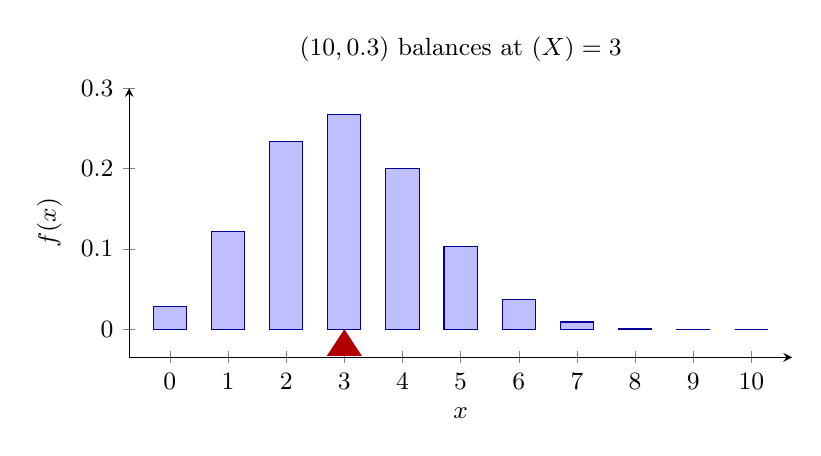
\begin{tikzpicture}
\begin{axis}[width=10cm, height=5cm, ybar, bar width=12pt, ymin=-0.035, ymax=0.3,
    xtick={0,...,10}, ytick={0,0.1,0.2,0.3}, xlabel={$x$}, ylabel={$f(x)$}, tick label style={font=\small}, label style={font=\small}, axis lines=left, scaled y ticks=false, yticklabel style={/pgf/number format/fixed},
    xmin=-0.7, xmax=10.7, axis x line=bottom, title={$\Bin(10,0.3)$ balances at $\E(X) = 3$},
    title style={font=\small}]
  \addplot[fill=blue!25, draw=blue!60!black] coordinates {(0,0.0282) (1,0.1211) (2,0.2335) (3,0.2668) (4,0.2001) (5,0.1029) (6,0.0368) (7,0.0090) (8,0.0014) (9,0.0001) (10,0.0000)};
  \fill[red!70!black] (axis cs:3,0) -- (axis cs:2.7,-0.033) -- (axis cs:3.3,-0.033) -- cycle;
\end{axis}
\end{tikzpicture}
\end{center}

\begin{example}[Fair die]
For one roll of a fair die, $\E(X) = \frac16(1+2+3+4+5+6) = 3.5$. The expected value need
not be a possible value of $X$.
\end{example}

\begin{example}[Lottery]
A $\$2$ ticket wins $\$1000$ with probability $0.001$ and $\$50$ with probability
$0.01$, otherwise nothing. The expected prize is
$1000(0.001) + 50(0.01) = 1 + 0.5 = \$1.50$, so the expected \emph{net} gain is
$1.50 - 2 = -\$0.50$ per ticket.
\end{example}

\section{Expectation of a function of a random variable}

\begin{theorem}[Law of the unconscious statistician]
If $X$ has p.f.\ $f(x)$ and $g$ is a function, then
\[
  \E[g(X)] = \sum_x g(x)\,f(x).
\]
\end{theorem}

\begin{proof}
Let $Y = g(X)$. Then $P(Y = y) = \sum_{x : g(x) = y} f(x)$, so
$\E(Y) = \sum_y y \sum_{x: g(x) = y} f(x) = \sum_x g(x) f(x)$, by regrouping the terms
of an absolutely convergent series.
\end{proof}

The point is that we never need to find the distribution of $g(X)$ to get its mean.

\begin{example}
For a fair die, $\E(X^2) = \frac16(1+4+9+16+25+36) = \frac{91}{6} \approx 15.17$. Note
$\E(X^2) \ne [\E(X)]^2 = 12.25$: in general $\E[g(X)] \ne g(\E X)$.
\end{example}

\begin{example}
If $X\sim\Poi(\mu)$, then
\[
  \E\left(\frac{1}{X+1}\right) = \sum_{x=0}^\infty \frac{1}{x+1}\cdot\frac{e^{-\mu}\mu^x}{x!}
  = \frac{e^{-\mu}}{\mu}\sum_{x=0}^\infty \frac{\mu^{x+1}}{(x+1)!}
  = \frac{e^{-\mu}}{\mu}(e^{\mu} - 1) = \frac{1 - e^{-\mu}}{\mu}.
\]
\end{example}

\begin{theorem}[Linearity]
For constants $a$, $b$ and functions $g_1$, $g_2$,
\[
  \E(aX + b) = a\E(X) + b, \qquad \E[a\,g_1(X) + b\,g_2(X)] = a\E[g_1(X)] + b\E[g_2(X)].
\]
\end{theorem}

\begin{proof}
$\sum_x (a g_1(x) + b g_2(x)) f(x) = a\sum_x g_1(x)f(x) + b \sum_x g_2(x)f(x)$; for the
first identity take $g_1(x) = x$, $g_2(x) = 1$ and use $\sum_x f(x) = 1$.
\end{proof}

\section{Variance and standard deviation}

\begin{definition}[Variance, standard deviation]
The \emph{variance} of $X$ is
\[
  \sigma^2 = \Var(X) = \E\left[(X - \mu)^2\right],
\]
the expected squared distance from the mean. The \emph{standard deviation} is
$\sigma = \SD(X) = \sqrt{\Var(X)}$, which has the same units as $X$.
\end{definition}


\begin{center}
\begin{tikzpicture}
\begin{axis}[name=a1, width=6.5cm, height=4.5cm, ybar, bar width=10pt, ymin=0, ymax=0.55,
    xmin=0.3, xmax=6.7, xtick={1,...,6}, xlabel={$x$}, ylabel={$f(x)$}, tick label style={font=\small}, label style={font=\small}, axis lines=left, scaled y ticks=false, yticklabel style={/pgf/number format/fixed},
    title={fair die: $\sigma^2 = 35/12$}, title style={font=\small}]
  \addplot[fill=blue!25, draw=blue!60!black] coordinates {(1,0.1667) (2,0.1667) (3,0.1667) (4,0.1667) (5,0.1667) (6,0.1667)};
  \draw[red!70!black, dashed] (axis cs:3.5,0) -- (axis cs:3.5,0.55);
\end{axis}
\begin{axis}[at={(a1.east)}, anchor=west, xshift=1cm, width=6.5cm, height=4.5cm, ybar,
    bar width=10pt, ymin=0, ymax=0.55, xmin=0.3, xmax=6.7, xtick={1,...,6}, xlabel={$x$}, tick label style={font=\small}, label style={font=\small}, axis lines=left, scaled y ticks=false, yticklabel style={/pgf/number format/fixed},
    title={$3$ or $4$, each w.p.\ $\tfrac12$: $\sigma^2 = 0.25$}, title style={font=\small}]
  \addplot[fill=orange!50, draw=orange!70!black] coordinates {(3,0.5) (4,0.5)};
  \draw[red!70!black, dashed] (axis cs:3.5,0) -- (axis cs:3.5,0.55);
\end{axis}
\end{tikzpicture}
\end{center}
Both distributions above have mean $3.5$ (dashed line), but the probability on the left is
much farther from the mean on average, so its variance is larger.

\begin{theorem}[Computing formulas]
\[
  \Var(X) = \E(X^2) - \mu^2 = \E[X(X-1)] + \mu - \mu^2.
\]
\end{theorem}

\begin{proof}
Expand: $\E[(X-\mu)^2] = \E(X^2) - 2\mu\E(X) + \mu^2 = \E(X^2) - \mu^2$. For the second,
$\E(X^2) = \E[X(X-1)] + \E(X)$.
\end{proof}

The form with $\E[X(X-1)]$ is convenient for distributions whose p.f.\ contains $x!$
(binomial, Poisson), because $x(x-1)/x! = 1/(x-2)!$ cancels nicely.

\begin{theorem}
$\Var(aX+b) = a^2\Var(X)$ and $\SD(aX+b) = \abs{a}\SD(X)$.
\end{theorem}

\begin{proof}
$aX + b - \E(aX+b) = a(X - \mu)$, so $\Var(aX+b) = \E[a^2(X-\mu)^2] = a^2\Var(X)$.
\end{proof}

Adding a constant shifts the distribution without changing its spread; scaling by $a$
scales the spread by $\abs a$.

\begin{example}[Fair die]
$\Var(X) = \frac{91}{6} - (3.5)^2 = \frac{182 - 147}{12} = \frac{35}{12} \approx 2.917$, so
$\sigma \approx 1.708$. If a game pays $Y = 10X - 20$ dollars, then
$\E(Y) = 10(3.5) - 20 = \$15$ and $\SD(Y) = 10\sigma \approx \$17.08$.
\end{example}

\section{Means and variances of the named distributions}

\begin{theorem}[Binomial]
If $X\sim\Bin(n,p)$, then $\E(X) = np$ and $\Var(X) = np(1-p)$.
\end{theorem}

\begin{proof}
Using $x\binom nx = n\binom{n-1}{x-1}$,
\[
  \E(X) = \sum_{x=1}^n n\binom{n-1}{x-1}p^x(1-p)^{n-x}
  = np\sum_{y=0}^{n-1}\binom{n-1}{y}p^y(1-p)^{n-1-y} = np,
\]
with $y = x - 1$ (the last sum is a $\Bin(n-1,p)$ total). Similarly
$x(x-1)\binom nx = n(n-1)\binom{n-2}{x-2}$ gives $\E[X(X-1)] = n(n-1)p^2$, so
\[
  \Var(X) = n(n-1)p^2 + np - n^2p^2 = np - np^2 = np(1-p).
\]
(A slicker proof using indicator variables appears in Chapter 8.)
\end{proof}

\begin{theorem}[Poisson]
If $X\sim\Poi(\mu)$, then $\E(X) = \Var(X) = \mu$.
\end{theorem}

\begin{proof}
\[
  \E(X) = \sum_{x=1}^\infty x\frac{e^{-\mu}\mu^x}{x!} = \mu e^{-\mu}\sum_{x=1}^\infty
  \frac{\mu^{x-1}}{(x-1)!} = \mu e^{-\mu}e^{\mu} = \mu,
\]
\[
  \E[X(X-1)] = \sum_{x=2}^\infty \frac{e^{-\mu}\mu^x}{(x-2)!} = \mu^2,
  \quad\text{so}\quad \Var(X) = \mu^2 + \mu - \mu^2 = \mu.
\]
\end{proof}

\begin{theorem}[Geometric and negative binomial]
If $X\sim\Geo(p)$, $\E(X) = \dfrac{1-p}{p}$ and $\Var(X) = \dfrac{1-p}{p^2}$. If
$X\sim\NB(k,p)$, $\E(X) = \dfrac{k(1-p)}{p}$ and $\Var(X) = \dfrac{k(1-p)}{p^2}$.
\end{theorem}

\begin{proof}[Proof (geometric mean)]
Let $q = 1-p$. Differentiating $\sum_{x\ge0} q^x = 1/(1-q)$ gives
$\sum_{x\ge1} xq^{x-1} = 1/(1-q)^2$. Hence
\[
  \E(X) = \sum_{x\ge 0} x p q^x = pq\sum_{x\ge1}xq^{x-1} = \frac{pq}{(1-q)^2} = \frac{q}{p}.
\]
Differentiating twice gives $\E[X(X-1)] = 2q^2/p^2$, so
$\Var(X) = 2q^2/p^2 + q/p - q^2/p^2 = (q^2 + pq)/p^2 = q/p^2$. The negative binomial is a
sum of $k$ independent geometrics (Chapter 8), so its mean and variance are $k$ times
these.
\end{proof}

\begin{theorem}[Hypergeometric]
If $X\sim\Hyp(N,r,n)$, then
\[
  \E(X) = \frac{nr}{N}, \qquad \Var(X) = n\frac{r}{N}\left(1-\frac rN\right)\frac{N-n}{N-1}.
\]
\end{theorem}

The mean matches the binomial with $p = r/N$; the variance is the binomial variance times
the \emph{finite population correction} $(N-n)/(N-1) < 1$ (sampling without replacement
is less variable). The proof is easiest with indicator variables (Chapter 8).

\begin{theorem}[Discrete uniform]
If $X$ is uniform on $\{a,\dots,b\}$, then $\E(X) = \dfrac{a+b}{2}$ and
$\Var(X) = \dfrac{(b-a+1)^2 - 1}{12}$.
\end{theorem}

For a die ($a=1$, $b=6$) this gives $3.5$ and $35/12$, as computed above.

\begin{example}
Applying these formulas to earlier examples:
\begin{itemize}
  \item $X\sim\Bin(10, 0.3)$: $\E(X) = 3$, $\Var(X) = 10(0.3)(0.7) = 2.1$.
  \item The fuse example ($N=20$, $r=5$, $n=5$): $\E(X) = 25/20 = 1.25$ and
        $\Var(X) = 5(0.25)(0.75)\cdot\frac{15}{19} \approx 0.7401$, compared with
        $0.9375$ for $\Bin(5, 0.25)$.
  \item Calls at rate $6$/hour for $20$ minutes: $\E(X) = \Var(X) = 2$.
\end{itemize}
\end{example}

\section{Chebyshev's inequality}

The standard deviation controls how much probability can lie far from the mean, whatever
the distribution.

\begin{theorem}[Chebyshev's inequality]
For any r.v.\ $X$ with mean $\mu$ and finite standard deviation $\sigma$, and any $k > 0$,
\[
  P(\abs{X - \mu} \ge k\sigma) \le \frac{1}{k^2}.
\]
\end{theorem}

\begin{proof}
Let $A = \{x : \abs{x-\mu}\ge k\sigma\}$. Then
\[
  \sigma^2 = \sum_x (x-\mu)^2 f(x) \ge \sum_{x\in A}(x-\mu)^2 f(x) \ge k^2\sigma^2
  \sum_{x\in A} f(x) = k^2\sigma^2 P(\abs{X-\mu}\ge k\sigma).
\]
\end{proof}

\begin{example}
At most $1/4$ of any distribution lies $2$ or more standard deviations from its mean,
and at most $1/9$ lies $3$ or more away. For a specific distribution (like the normal)
the true probabilities are usually much smaller (about $0.046$ and $0.003$).
\end{example}

\begin{center}
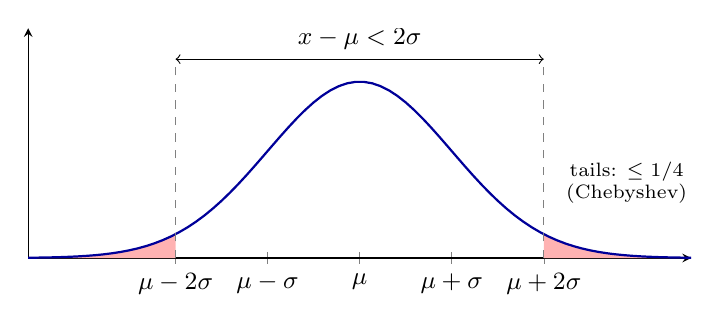
\begin{tikzpicture}
\begin{axis}[width=10cm, height=4.5cm, xmin=-3.6, xmax=3.6, ymin=0, ymax=0.52,
    xtick={-2,-1,0,1,2}, xticklabels={$\mu-2\sigma$,$\mu-\sigma$,$\mu$,$\mu+\sigma$,$\mu+2\sigma$},
    ytick=\empty, axis lines=left, tick label style={font=\small}, samples=80]
  \addplot[draw=none, fill=red!30, domain=-3.6:-2] {exp(-x^2/2)/sqrt(2*pi)} \closedcycle;
  \addplot[draw=none, fill=red!30, domain=2:3.6] {exp(-x^2/2)/sqrt(2*pi)} \closedcycle;
  \addplot[thick, blue!60!black, domain=-3.6:3.6] {exp(-x^2/2)/sqrt(2*pi)};
  \draw[dashed, gray] (axis cs:-2,0) -- (axis cs:-2,0.45);
  \draw[dashed, gray] (axis cs:2,0) -- (axis cs:2,0.45);
  \node[font=\scriptsize, align=center] at (axis cs:2.9,0.17) {tails: $\le 1/4$\\(Chebyshev)};
  \draw[<->] (axis cs:-2,0.45) -- node[above, font=\small] {$\abs{x-\mu} < 2\sigma$} (axis cs:2,0.45);
\end{axis}
\end{tikzpicture}
\end{center}
Chebyshev bounds the shaded tail area by $1/k^2$ for \emph{every} distribution; for the
normal curve drawn here the true area is only about $0.046$.

\section{Common pitfalls}

\begin{itemize}
  \item $\E[g(X)] \ne g(\E X)$ in general, e.g.\ $\E(X^2) \ne (\E X)^2$ and
        $\E(1/X) \ne 1/\E(X)$.
  \item $\Var(aX + b) = a^2\Var(X)$: the constant disappears and $a$ is squared;
        $\Var(-X) = \Var(X)$.
  \item Check which convention is used for the geometric: failures before the first
        success has mean $(1-p)/p$; total trials has mean $1/p$.
\end{itemize}

\section{Summary}

\begin{itemize}
  \item $\E(X) = \sum x f(x)$; $\E[g(X)] = \sum g(x) f(x)$; expectation is linear.
  \item $\Var(X) = \E[(X-\mu)^2] = \E(X^2) - \mu^2 = \E[X(X-1)] + \mu - \mu^2$.
  \item $\Var(aX+b) = a^2\Var(X)$.
  \item Binomial $np$, $np(1-p)$; Poisson $\mu$, $\mu$; geometric $q/p$, $q/p^2$;
        negative binomial $kq/p$, $kq/p^2$; hypergeometric $nr/N$ with the finite
        population correction.
  \item Chebyshev: $P(\abs{X-\mu}\ge k\sigma)\le 1/k^2$.
\end{itemize}
